\question{4.4}{Het aantal augurken dat in een halveliterpot zit, blijkt enigszins te vari\"eren. Uitvoerig onderzoek heeft aangetoond dat dit aantal tussen 15 en 20 ligt, waarbij de volgende kansen van toepassing zijn:}
\begin{center}
    \begin{tabular}{ccccccc}
        \toprule
            {\bfseries Aantal augurken $k$} & $15$ & $16$ & $17$ & $18$ & $19$ & $20$\\
        \cmidrule{1-1} \cmidrule{2-2} \cmidrule{3-3} \cmidrule{4-4} \cmidrule{5-5} \cmidrule{6-6} \cmidrule{7-7}
            $P(X = k)$ & $0,10$ & $0,30$ & $0,30$ & $0,15$ & $0,10$ & $0,05$\\
        \bottomrule
    \end{tabular}
\end{center}

\begin{enumerate}[label=(\alph*)]
    \item Teken de kansfunctie
    \answer{
        \begin{center}
            \resizebox{0.9\textwidth}{!}{
                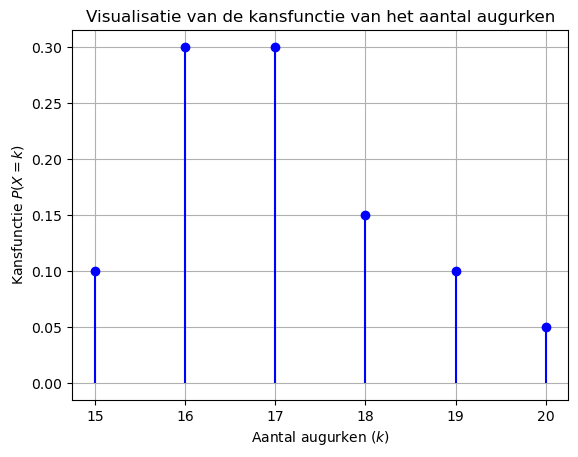
\includegraphics{opg4.4a.png}
            }
        \end{center}
    }

    \item Bereken en teken de cumulatieve kansfunctie. 
    \answer{
        We beschreven $F$, de cumulatieve verdelingsfunctie (CDF), door middel van een tabel:
        \begin{center}
            \begin{tabular}{ccccccc}
                \toprule
                    {\bfseries Aantal augurken $k$} & $15$ & $16$ & $17$ & $18$ & $19$ & $20$\\
                \cmidrule{1-1} \cmidrule{2-2} \cmidrule{3-3} \cmidrule{4-4} \cmidrule{5-5} \cmidrule{6-6} \cmidrule{7-7}
                    $F(k)=P(X \le k)$ & $0,10$ & $0,40$ & $0,70$ & $0,85$ & $0,95$ & $1,00$\\
                \bottomrule
            \end{tabular}
        \end{center}

        In een grafiekvorm ziet dit er als volgt uit:
        
        \begin{center}
            \resizebox{0.9\textwidth}{!}{
                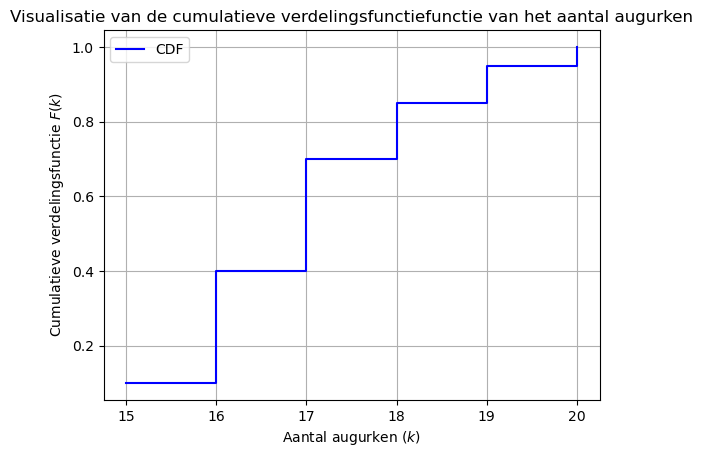
\includegraphics{opg4.4b.png}
            }
        \end{center}
    }

    \item Hoe groot is de kans om in een willekeurige pot meer dan 16 maar minder dan 20 augurken aan te treffen?
    \answer{
        We willen de kans $P(16 < X < 20)$ bepalen. Omdat we met een discrete verdeling werken, kunnen we die als volgt berekenen:
        \[
            P(16 < X < 20) = P(17 \le X \le 19) = F(19) - F(16) = 0,95 - 0,40 = 0,55.
        \]
    }  

    \item Er worden twee willekeurige potten augurken geselecteerd.
    Hoe groot is de kans dat beide potten meer dan 18 augurken bevatten?
    \answer{
        Als er twee willekeurige potten geselecteerd zijn, dan geldt dat beide met kans $P(X > 18) = 1 - P(X \le 18) = 1 - 0,85 = 0,15$ meer dan 18 augurken bevatten.
        Omdat de potten onafhankelijk van elkaar gevuld zijn, is de totale kans gelijk aan $0,15 \cdot 0,15 = 0,0225$.
    }  

    \item Hoe groot is de kans dat twee willekeurige potten augurken in totaal 38 augurken bevatten.
    \answer{
        Laat nu $X_1$ het aantal augurken zijn in pot 1, en $X_2$ het aantal augurken in pot 2.
        We willen de kans $P(X_1+X_2=38)$ bepalen. Dit doen we als volgt:
        \begin{align*}
            P(X_1+X_2=38) &= P(X_1 = 18, X_2=20) + P(X_1 = 19, X_2=19) \\
                          &\qquad + P(X_1 = 20, X_2=18) \\
                          &= 0,15 \cdot 0,05 + 0,10 \cdot 0,10 + 0,05 \cdot 0,15 \\
                          &= 0,025.
        \end{align*}
        Met $2,5\%$ kans is het totaal aantal augurken in twee willekeurige potten samen gelijk aan 38.
    }
    \end{enumerate}